\documentclass{article}
\title{Electromagnetism Practical, Session 1\\Transmission Lines}
\author{Rijk van Wijk 0000000, Bart Kolling 4228219, Chy Lau 0000000,\\ Jasper Smit 4217527, Ian Zhang 0000000}
\usepackage{graphicx}
\usepackage{float}

\usepackage[square,numbers]{natbib}

\begin{document}
	\maketitle
	\section*{Assignment 1: Transmission Lines in Frequency Domain}
	\subsection*{Part 1: Standing Waves in Waveguide}
	% de wavelength = afstand tussen 2 knopen * 2 = 2.2*2 = 4.4cm. de phase velocity kwam uit op 1.39c, weet niet meer waarom. 
	% bij shortcut 33mm komt hetzelfde uit als bij shortcut 55mm.
	% also, er is blijkbaar geen part 2? w/e.. doei, jasper.
	The measured wavelength of the standing wave is 4.4 cm. The phase velocity is determined by equation \ref{eq1}. The wavelength in the waveguide is determined by equation \ref{eq2} with an a of 22.86 mm at a frequency of 9.475 GHz. The result is that the phase velocity is $v = 1.39c$. This is the case because the wavelength is modified inside the waveguide.
	\begin{equation}
	\label{eq1}
	v_p = \frac{\lambda}{T}
	\end{equation}
	\begin{equation}
	\label{eq2}
	\lambda _w = \frac{\lambda _0}{\sqrt{1 - (\frac{\lambda _0}{2a})^2}}
	\end{equation}
	
	\subsection*{2.}
	The voltage-standing-wave ratio (VSWR) of different loads is measured.
	\subsubsection*{a.}
The open waveguide 
	
	\subsubsection*{b.}
	Both the short circuits give a minimum of 0.02 mV and a maximum of 80 mV. This gives a VSWR of about $4.0 \cdot 10^3$.
	
	\subsubsection*{c.}
	The matched load gives a minimum of 45.4 mV and a maximum of 50.3 mV giving a VSWR of 1.11.
	
	\subsubsection*{d.}
	The horn antenna gives a minimum of 45.2 mV and a maximum of 51.1 mV. This gives a VSWR of 1.13.
	
	\subsection*{3.}
	There is no shift in antinodes in our measurement regarding the two short-circuits. This is not surprising as the difference between the 33mm and the 55mm short-circuit is exactly 22mm which is half of the wavelength.
	
	\subsection*{Additional Tasks}
	The dependence of the phase velocity on the wavelength can be calculated using equation \ref{eq1}. This gives the result in figure \ref{fig1}.
	
	\begin{figure}[H]
	\centering
	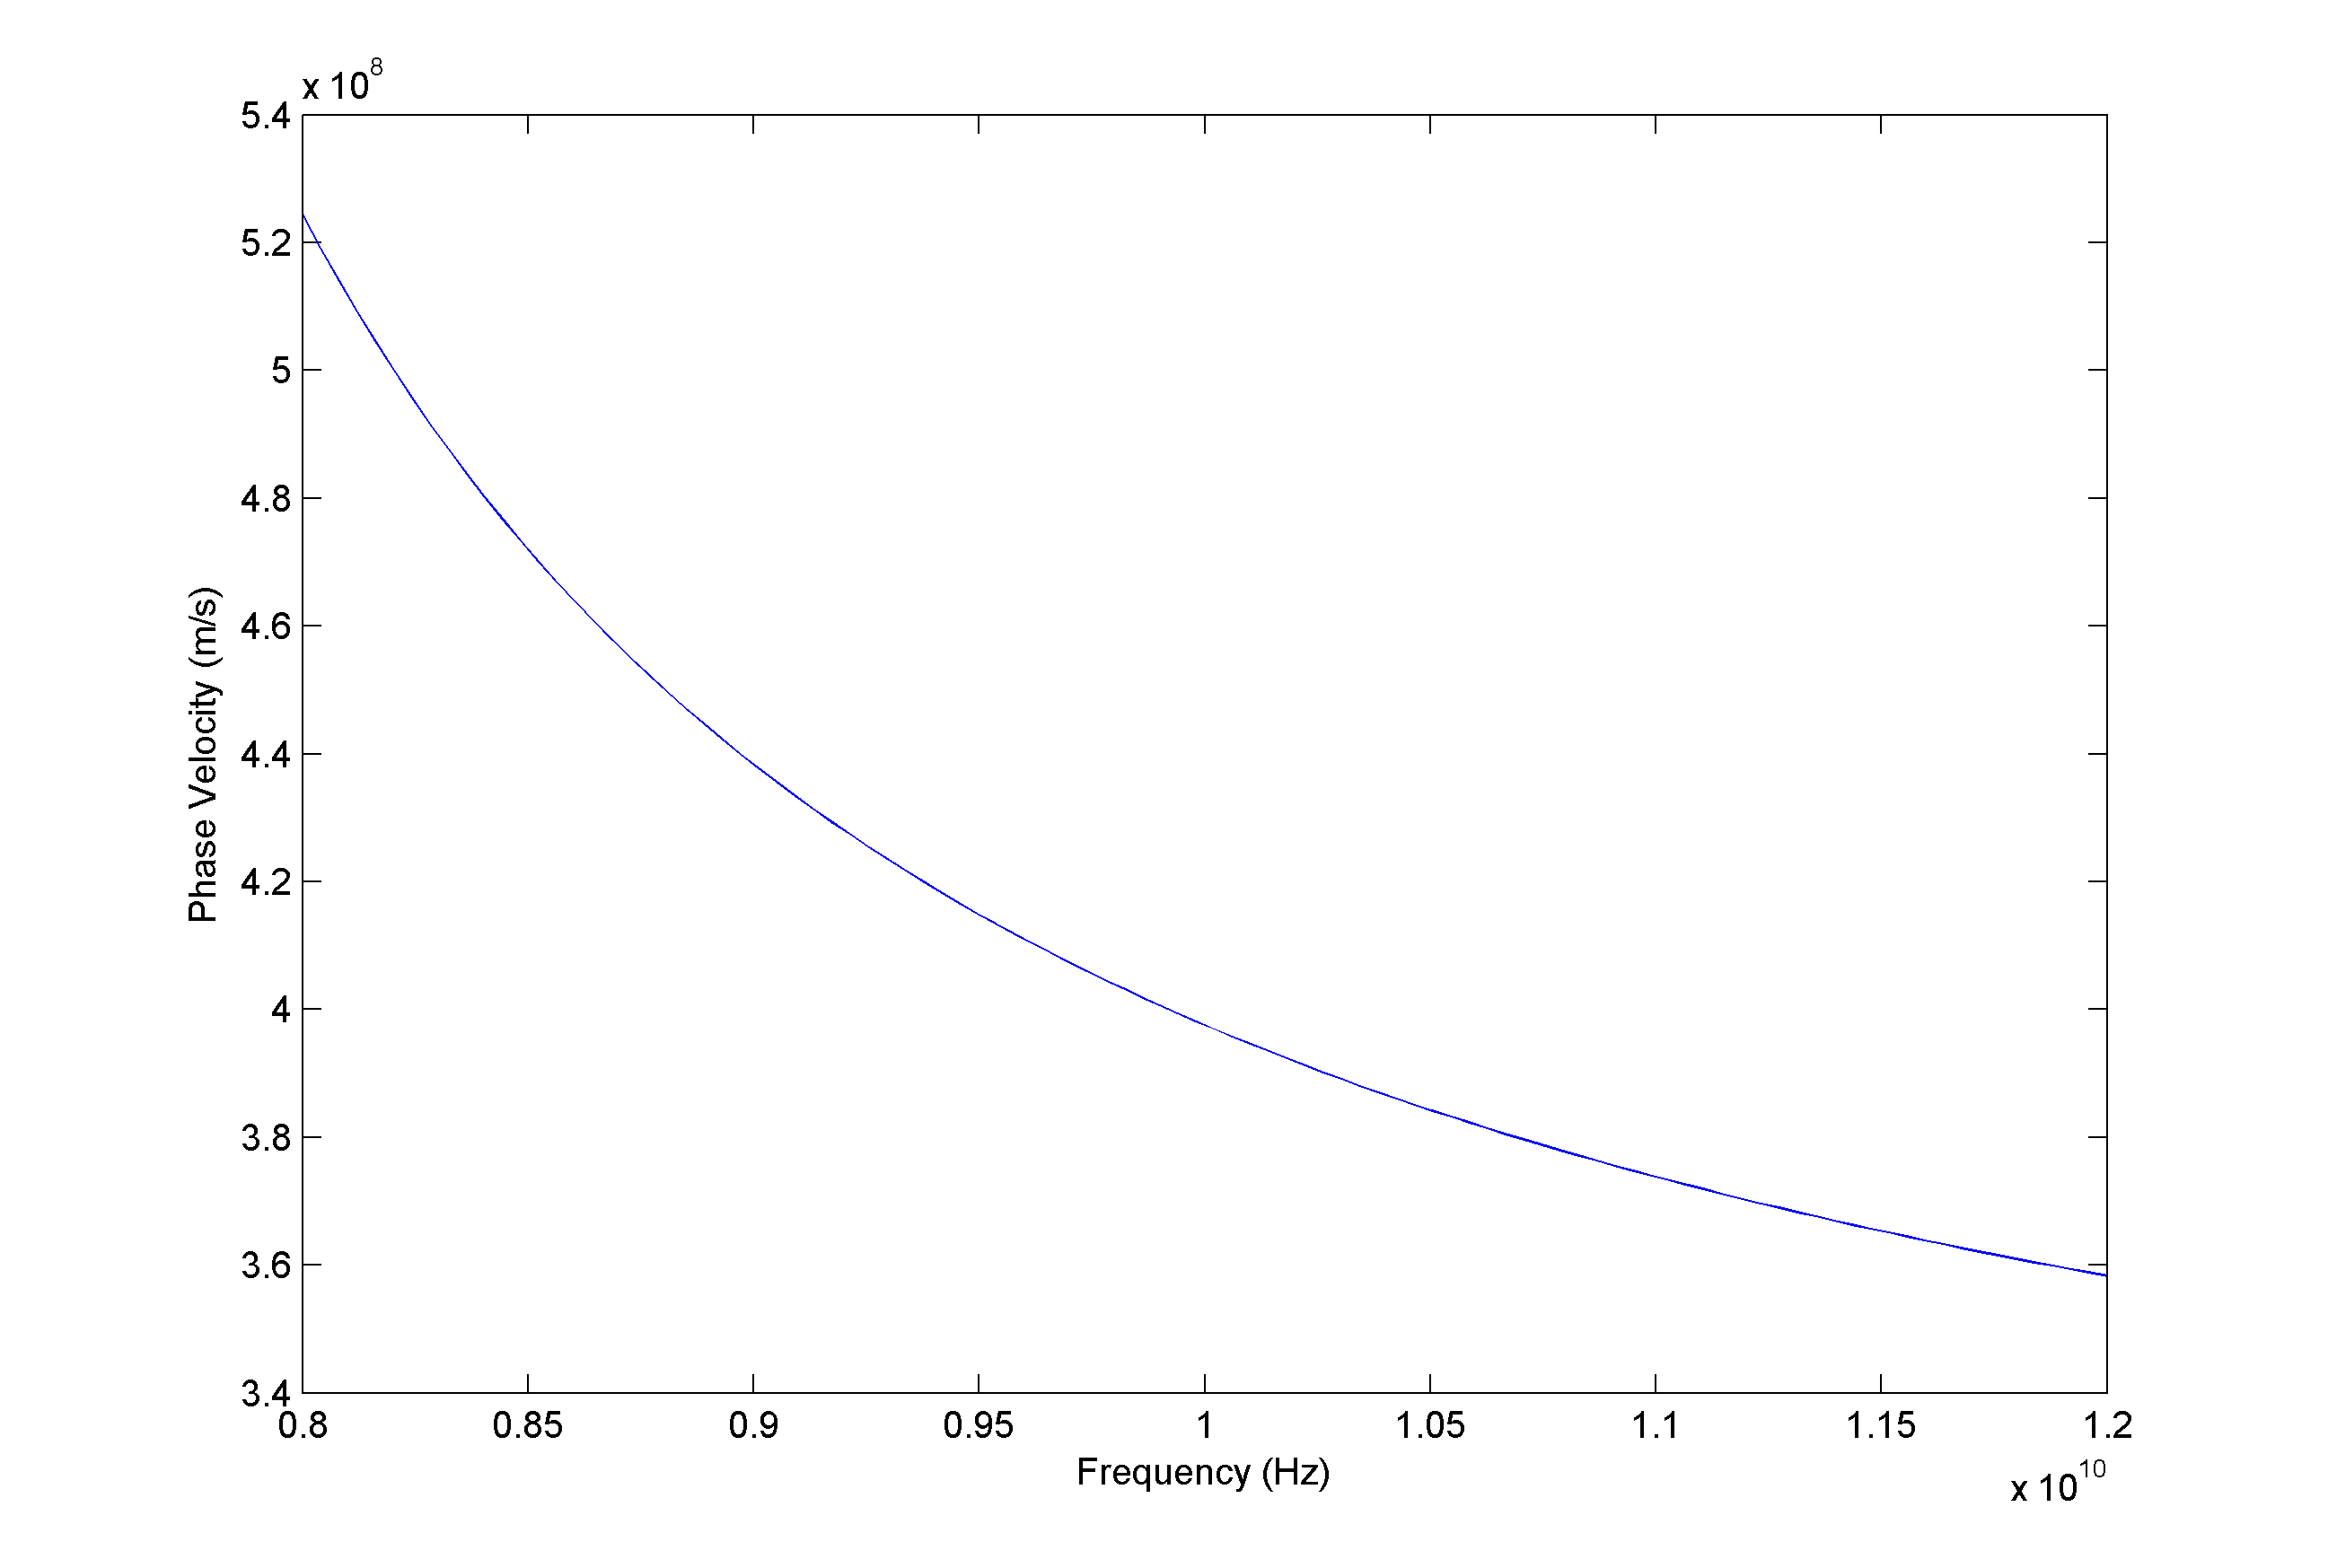
\includegraphics[width=\textwidth]{plotjes/phasevel.png}
	\caption{The phase velocity in the x-band.}
	\label{fig1}
	\end{figure}
	
	Other parameters that can be estimated using the measurements are
	
	
	
	\section*{Assignment 2: Transmission Lines in Time Domain}
		\subsection*{Part 1: Time Domain Reflectometry: estimate the load’s impedance}
			$Z_l$ can be determined with equation \ref{zload}. The voltage standing wave ration is measured as $VSWR = \rho = 0.2$ and our $Z_0 = 50 \Omega$
			\begin{equation}
			\label{zload}
				\rho = \frac{Z_l-Z_0}{Z_l+Z_0}
			\end{equation}
			\begin{equation}
				Z_l = - \frac{\rho + 1}{\rho - 1} \cdot Z_0 = 75 \Omega
			\end{equation}
	
		\subsection*{Part 2:  Dielectric in Coaxial Cable: the Estimation of the Propagation Speed and Relative Permittivity}
			From the reflections the propagation velocity turned out to be $0.77c$, which is exactly what the datasheet of the cable states\cite{datasheetcable}. 
			Using equation \ref{propvel} the relative permittivity $\epsilon_r$ can be calculated.
			\begin{equation}
			\label{propvel}
				v = \frac{c}{\sqrt{\epsilon_r}} = 0.77 c
			\end{equation}
			\begin{equation}
				\epsilon_r = (\frac{c}{v})^2 = 1.69
			\end{equation}


	\clearpage
	\bibliographystyle{plainnat}
	\bibliography{bib}
\end{document}
